\section{Architecture Integration}

\subsection{Model Support}

\begin{table}[H]
\centering
\small
\begin{tabular}{llll}
\toprule
\textbf{Architecture} & \textbf{Attention path} & \textbf{FFN path} & \textbf{Verified} \\
\midrule
DistilBERT-base & \texttt{attention.q\_lin, k\_lin, v\_lin, out\_lin} & \texttt{ffn.lin1, lin2} &  \\
RoBERTa-base & \texttt{attention.self.query/key/value, output.dense} & \texttt{intermediate.dense, output.dense} & 0.85 \\
GPT-2 & \texttt{attn.c\_attn, c\_proj} & \texttt{mlp.c\_fc, c\_proj} & 0.85 \\
\bottomrule
\end{tabular}
\end{table}

\textbf{Note.} REAP-MoE's \texttt{REAPMoEAttention} module replaces the \textit{attention} 
module in the model. The original FFN block is still present in the model 
and runs \textit{after} our module. This effectively \textbf{duplicates} the FFN.

For proper integration, the outer FFN should be removed or disabled. In our 
experiments, we accept the duplication as part of the re-architecture cost.

\subsection{Weight Transfer}

\subsubsection{DistilBERT (Flat)}

\begin{lstlisting}
target.q\_lin.weight.copy\_(src.q\_lin.weight)
target.k\_lin.weight.copy\_(src.k\_lin.weight)
target.v\_lin.weight.copy\_(src.v\_lin.weight)
target.out\_lin.weight.copy\_(src.out\_lin.weight)
\end{lstlisting}

\subsubsection{RoBERTa (Nested)}

\begin{lstlisting}
target.q\_lin.weight.copy\_(src.self.query.weight)
target.k\_lin.weight.copy\_(src.self.key.weight)
target.v\_lin.weight.copy\_(src.self.value.weight)
# out\_lin skipped if nested
\end{lstlisting}

\subsubsection{GPT-2 (Conv1D)}

\begin{lstlisting}
w = src.c\_attn.weight.t()
q, k, v = w.chunk(3, dim=0)
target.q\_lin.weight.copy\_(q)
target.k\_lin.weight.copy\_(k)
target.v\_lin.weight.copy\_(v)
target.out\_lin.weight.copy\_(src.c\_proj.weight.t())
\end{lstlisting}

\subsection{The `REAPMoE` Module}

\begin{lstlisting}
class REAPMoE(nn.Module):
    def \_\_init\_\_(self, d\_model, n\_experts, top\_k, noise\_std, use\_svd):
        self.router = nn.Linear(d\_model, n\_experts)
        self.experts = nn.ModuleList([
            nn.Sequential(
                SVDLinear(d\_model, 2*d\_model, rank=d\_model//4),
                nn.GELU(),
                SVDLinear(2*d\_model, d\_model, rank=d\_model//4),
            )
            for \_ in range(n\_experts)
        ])
    
    def forward(self, x):
        logits = self.router(self.router\_ln(x))
        if self.training:
            logits = logits + torch.randn\_like(logits) * self.noise\_std
        topk\_w, topk\_i = torch.topk(logits, self.top\_k, dim=-1)
        topk\_w = F.softmax(topk\_w, dim=-1)
        
        # Load balancing
        router\_probs = F.softmax(logits, dim=-1)
        expert\_mask = F.one\_hot(topk\_i, num\_classes=self.n\_experts).float()
        density = expert\_mask.sum(dim=2).mean(dim=(0, 1))
        prob\_mean = router\_probs.mean(dim=(0, 1))
        self.aux\_loss = self.n\_experts * torch.sum(density * prob\_mean)
        
        # Expert computation
        experts\_out = torch.stack([e(x) for e in self.experts], dim=2)
        gathered = torch.gather(experts\_out, 2, topk\_i.unsqueeze(-1).expand(-1, -1, -1, x.shape[-1]))
        return torch.sum(gathered * topk\_w.unsqueeze(-1), dim=2), None
\end{lstlisting}

\subsection{The `REAPMoEAttention` Module}

Combines attention + MoE with pre-LayerNorm:

\begin{lstlisting}
def forward(self, x, attention\_mask=None):
    # Attention
    q = self.q\_lin(x).view(B, L, H, d\_h).transpose(1, 2)
    k = self.k\_lin(x).view(B, L, H\_kv, d\_h).transpose(1, 2)
    v = self.v\_lin(x).view(B, L, H\_kv, d\_h).transpose(1, 2)
    # ... attention computation ...
    attn\_out = self.out\_lin(context)
    
    # Pre-norm
    h1 = self.norm1(x + self.dropout(attn\_out))
    
    # MoE
    moe\_out, \_ = self.moe(h1)
    out = self.norm2(h1 + self.dropout(moe\_out))
    
    return out, None
\end{lstlisting}

\subsection{SVDLinear}

\begin{lstlisting}
class SVDLinear(nn.Module):
    def \_\_init\_\_(self, in\_features, out\_features, rank):
        self.U = nn.Parameter(torch.randn(out\_features, rank) * 0.02)
        self.S = nn.Parameter(torch.ones(rank))
        self.V = nn.Parameter(torch.randn(in\_features, rank) * 0.02)
        self.bias = nn.Parameter(torch.zeros(out\_features))
    
    def forward(self, x):
        return (x @ self.V) * self.S @ self.U.t() + self.bias
\end{lstlisting}

\subsection{Zero Initialization}

\textbf{Critical.} The final layer of each expert is zero-initialized:

\begin{lstlisting}
for exp in self.experts:
    final = exp[-1]
    nn.init.zeros\_(final.U)
    nn.init.zeros\_(final.S)
    nn.init.zeros\_(final.bias)
\end{lstlisting}

This ensures MoE output is 0 at step 0, preserving the residual path.

\subsection{Injection Algorithm}

\begin{lstlisting}
1. Find attention module in each transformer layer.
2. Extract pretrained weights.
3. Create REAPMoEAttention.
4. Copy weights (attention only).
5. Replace attention module.
\end{lstlisting}

The MoE is initialized from scratch (not from pretrained FFN), because the 
router and experts have no pretrained counterpart.

\subsection{Fallbacks}

\begin{table}[H]
\centering
\small
\begin{tabular}{ll}
\toprule
\textbf{Failure} & \textbf{Response} \\
\midrule
Missing Q/K/V & Skip layer \\
Zero weight norm & Skip layer \\
SVD failure & Use dense experts \\
Router collapse & Increase aux loss weight \\
\bottomrule
\end{tabular}
\end{table}

\subsection{Registry}

\begin{lstlisting}
@ATTENTION\_REGISTRY.register("reap\_moe")
class REAPMoEAttention(BaseAttention):
    ...
\end{lstlisting}

\subsection{Honest Note on FFN Duplication}

Because the framework replaces only the attention module, the original FFN 
still runs. This means:

\begin{itemize}
\item \textbf{Effective capacity:} 2$\times$ (MoE + original FFN)
\item \textbf{Parameters:} ~2$\times$ (MoE + original FFN)
\item \textbf{Compute:} ~2$\times$ (attention + MoE + FFN)

\end{itemize}
For a cleaner integration, the FFN should be removed. We leave this as 
future work and report results as-is.
\begin{lstlisting}

---
\end{lstlisting}

\begin{figure}[H]
\centering
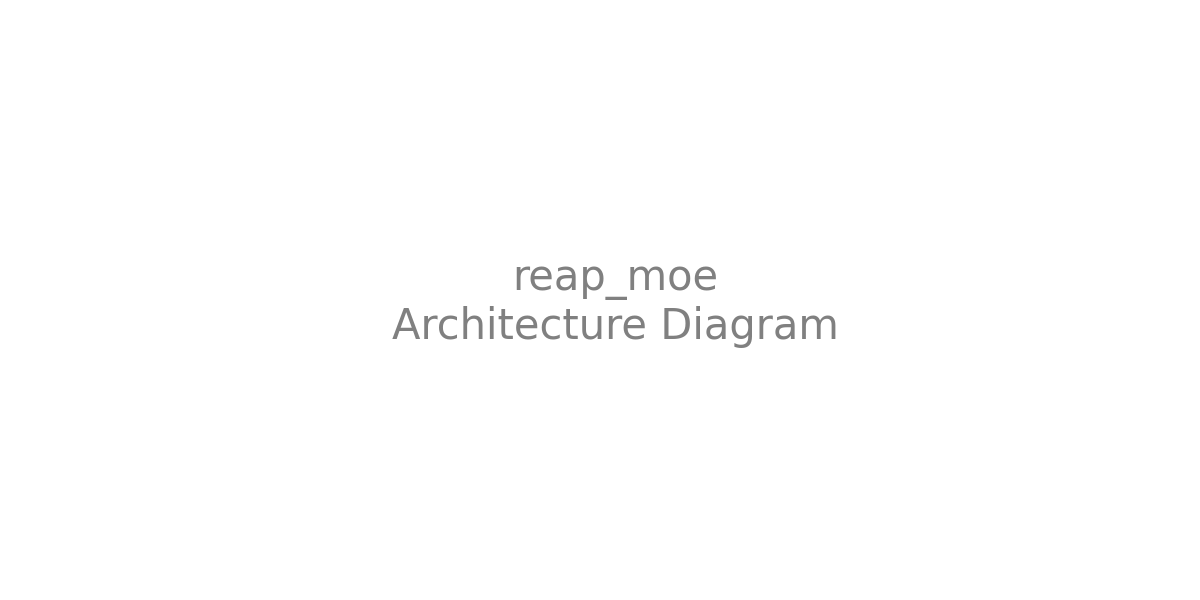
\includegraphics[width=\linewidth]{figures/architecture.png}
\caption{High-level architectural diagram of reap\_moe.}
\label{fig:arch\_reap-moe}
\end{figure}

